% ============================================================================
% A7 v2 figures and tables (R018). Generated by figures/gen_*.py from experiments/a7/results/.
% Caption numbers trace to: main_summary.json, m2m3_summary.json, r019_derived.json, scaling.csv, figures/fig1_values.json.
% Claim scope: CLAIMS_FROM_RESULTS.md. Revised after the GPT-6 Astra figure review (2026-09-28).
% Draft captions; /paper-write may shorten them.
% ============================================================================

% === Fig. 1: geometry and certificate construction (full width) ===
\begin{figure*}[t]
  \centering
  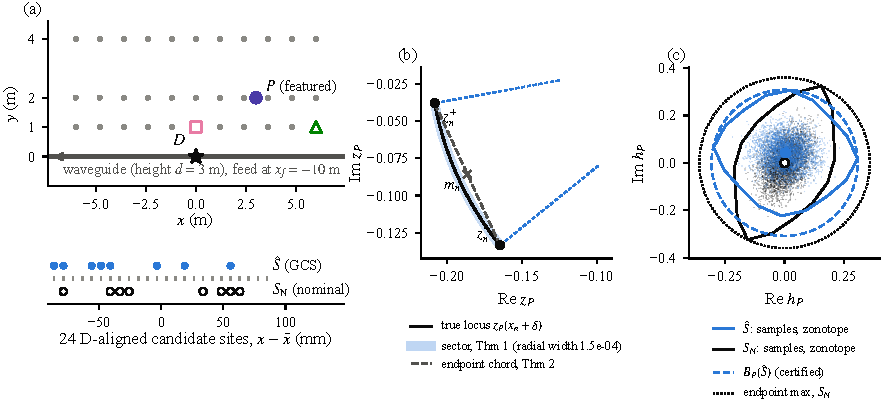
\includegraphics[width=\textwidth]{figures/fig1_geometry.pdf}
  \caption{Geometry and certificate construction for the featured case (free family, $P = (3, 2)$~m,
  $\epsilon = 0.05\lambda$, 30~dB). (a)~Top view (coordinates in metres): waveguide along $x$ (height $d = 3$~m, feed at
  $x_f = -10$~m), desired receiver $D$, the 33 main-grid protected positions (gray), the tolerance-sweep positions $(6,1)$
  and $(0,1)$ of Fig.~\ref{fig:limits} (hollow), and the featured position $(3,2)$ (filled, not on the grid); below, the 24
  D-aligned candidate sites with the GCS layout $\hat S$ and the exhaustive nominal layout $S_{\rm N}$. (b)~One selected
  site: the true contribution $z_P(x_n+\delta)$, $|\delta| \le \epsilon$, inside its asymmetric sector (Theorem~1; true
  radial width $1.5\times10^{-4}$ relative, band widened for visibility) and the endpoint chord that generates the
  zonotope (Theorem~2). (c)~Leakage field $h_P$ under 4000 uniform error draws per layout, the endpoint zonotopes, and the
  nominal fields (filled: $\hat S$, $|h_P| = 0.043$; hollow: $S_{\rm N}$, $|h_P| = 3.4\times10^{-4}$, a deep null). The
  certified bound $B_P(\hat S)$ (dashed circle) and the endpoint witness of $S_{\rm N}$ (dotted circle) order the worst
  cases, with bounds rounded outward:
  $\max_\delta |h_P(\hat S,\delta)| \le 0.3081 < 0.3596 \le \max_\delta |h_P(S_{\rm N},\delta)|$.}
  \label{fig:geometry}
\end{figure*}

% === Fig. 2: certified gain distributions (full width) ===
\begin{figure*}[t]
  \centering
  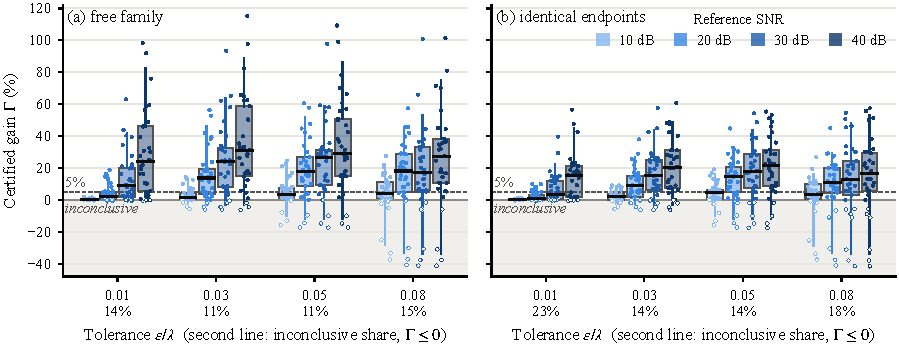
\includegraphics[width=\textwidth]{figures/fig2_gamma.pdf}
  \caption{Certified gain $\Gamma = L(\hat S)/U(S_{\rm N}) - 1$ of GCS over the exhaustive nominal layout on the declared
  grid ($\epsilon > 0$, $P \neq D$), (a)~free family, (b)~identical endpoints. Within each tolerance, boxes from left to
  right are reference SNR 10, 20, 30, 40~dB; each box summarizes the 33 protected positions: box = interquartile range,
  bar = median, whiskers = 5th--95th percentiles, dots = cases (hollow: $\Gamma \le 0$). $\Gamma > 0$ certifies a higher
  worst-case SLNR; $\Gamma \le 0$ (gray band) means the certificate is inconclusive, not that the robust layout is worse.
  Second tick line: inconclusive share per tolerance (132 cases). Dashed line: the pre-declared 5\% level. Over the 528
  cases per family, $\Gamma > 0$ in 87.5\% (free) and 82.8\% (endpoints).}
  \label{fig:gamma}
\end{figure*}

% === Fig. 3: tolerance sweep, protection limits (single column) ===
\begin{figure}[t]
  \centering
  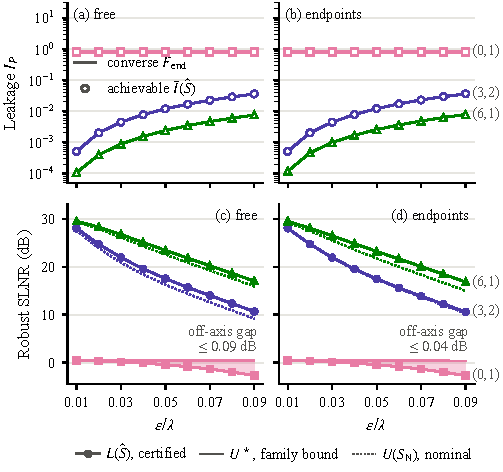
\includegraphics[width=\columnwidth]{figures/fig3_limits.pdf}
  \caption{Tolerance sweep at 30~dB for three pre-specified protected positions (in metres) and both families (54 cases).
  (a,b)~Leakage power $I_P = |\sum_{n\in S} z_P(x_n+\delta_n)|^2/N$: family-wide endpoint converse
  $F_{\rm end} \le \min_S \max_\delta I_P$ (lines) and the certified leakage bound $\bar I(\hat S)$ of the selected layout
  (markers); they agree within 1.14\% at every point. At transmit power $p$, no layout of the family meets a leakage
  ceiling $I_{\max} < pF_{\rm end}$ for all errors; for $P = (0, 1)$, behind $D$, $F_{\rm end} \approx 0.80$ at every
  $\epsilon$. (c,d)~Certified SLNR lower bound $L(\hat S)$, the family upper bound $U^\star$ (thin line; shaded bracket),
  and the upper witness $U(S_{\rm N})$ of the exhaustive nominal layout (dotted). The printed off-axis gap is
  $\max 10\log_{10}[U^\star/L(\hat S)]$ over $P \in \{(3,2), (6,1)\}$. $L(\hat S)$ above $U(S_{\rm N})$ certifies
  dominance; for $P = (0, 1)$ the comparison is inconclusive.}
  \label{fig:limits}
\end{figure}

% === Fig. 4: screening efficiency (single column) ===
\begin{figure}[t]
  \centering
  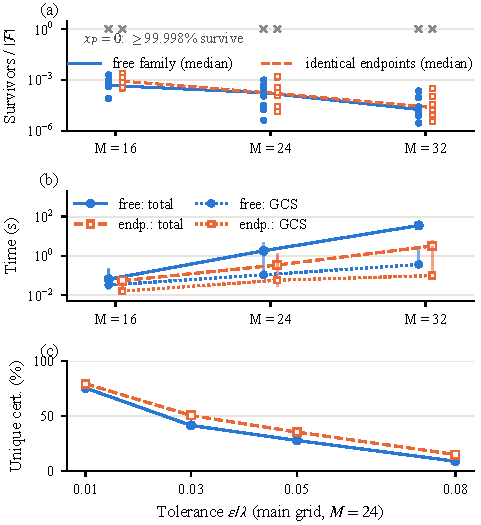
\includegraphics[width=\columnwidth]{figures/fig4_screening.pdf}
  \caption{Global screening. (a)~Fraction of the family surviving safe screening for $M \in \{16, 24, 32\}$ candidate
  sites ($N = 8$; 6 pre-declared positions $\times$ $\epsilon/\lambda \in \{0.03, 0.05\}$ at 30~dB, 12 cases per family and
  $M$; $|\mathcal F|$ up to $1.05 \times 10^{7}$). Lines: median over the 8 cases with $x_P \neq 0$; $\times$: the 4 cases
  with $P$ behind $D$ ($x_P = 0$), where at least 99.998\% of the family survives and the screening cap is hit for
  $M \ge 24$ (free) and $M = 32$ (endpoints). (b)~Wall time per case, median of 12 (bars: range): total (setup, family
  construction, endpoint-bank pass, nominal enumeration, screening, nominal-witness refinement) and the GCS selection stage
  (``GCS''; ``endp.'' = identical endpoints); capped scans are included as run. (c)~Share of cases with a unique robust-optimality certificate within the respective
  finite family (main grid, $M = 24$; 33 positions $\times$ 4 SNRs $= 132$ per point and family, $P = D$ excluded).}
  \label{fig:screening}
\end{figure}

% === Table I: protocol ===
\begin{table}[t]
\centering
\caption{Simulation protocol (declared before the runs).}
\label{tab:protocol}
\footnotesize
\begin{tabular}{@{}p{0.24\columnwidth}p{0.70\columnwidth}@{}}
\toprule
Carrier, wavelength & $f_c = 28$ GHz, $\lambda = 10.714$ mm \\
Waveguide & $n_{\rm eff} = 1.44$, height $d = 3$ m, feed $x_f = -10$ m \\
Candidate family & $M = 24$ D-aligned sites, select $N = 8$, $d_{\min} = 0.5\lambda$ \\
Receivers & $D = (0,0)$; 33 positions $P$ ($x_P$: 11 values in $[-6, 6]$ m; $y_P \in \{1,2,4\}$ m) and the control $P = D$ \\
Tolerance & $\epsilon/\lambda \in \{0, 0.01, 0.03, 0.05, 0.08\}$ \\
Reference SNR & $\{10, 20, 30, 40\}$ dB, relative to the central 8-site block toward $D$; fixed physical noise per SNR \\
Families & free; identical endpoints (sites 1 and $M$ forced) \\
Certificates & $K = 1440$ with $\sec(\pi/K)$; $\beta_D \le \pi/2$ guard \\
Witnesses & $\le 2M$ family-wide endpoint templates (screening); for $S_{\rm N}$ / $\hat S$: all $2^N$ corners + 4 / 8 L-BFGS-B starts \\
Search & swap from $S_{\rm N}$ + 8 random starts (seed 2026); screening cap $2\times10^{5}$ evaluations \\
Main grid & 1360 cases (2 families $\times$ 4 SNR $\times$ 5 $\epsilon$ $\times$ 34 positions) \\
\bottomrule
\end{tabular}
\end{table}


% === Table II: results summary ===
\begin{table}[t]
\centering
\caption{Certified results. $\Gamma = L(\hat S)/U(S_{\rm N}) - 1$; $\Gamma > 0$ certifies a higher worst-case SLNR than the
exhaustive nominal layout in the same family. Certificates are analytical; all inequalities are evaluated in float64.
Rival margin: $L(\hat S) - \max_{S \neq \hat S} U_H(S)$. B-GR: desired-only, P-blind layout.
$^\dagger$Same-start shared-template swap heuristic (budgets not matched). $^\ddagger$Waveguide attenuation plus
$\cos^2\theta$ field directivity; both layouts redesigned under the model at a model-specific reference SNR.}
\label{tab:results}
\footnotesize
\setlength{\tabcolsep}{3pt}
\begin{tabular}{@{}lrr@{}}
\toprule
 & Free & Endpoints \\
\midrule
\multicolumn{3}{@{}p{0.97\columnwidth}}{\emph{Main grid, $\epsilon > 0$, $P \neq D$ ($n = 528$ per family), vs.\ exhaustive nominal $S_{\rm N}$}} \\
$\Gamma > 0$ (cert.\ dominance) & 87.50\% (462) & 82.77\% (437) \\
$\Gamma > 5\%$ & 61.93\% (327) & 56.25\% (297) \\
Median $\Gamma$ [IQR] & 11.3 [1.6, 27.6]\% & 6.9 [0.5, 19.4]\% \\
Inconclusive ($\Gamma \le 0$) & 12.5\% & 17.2\% \\
Median nominal sacrifice & 0.16\% & 0.32\% \\
Unique robust optimum & 38.6\% & 45.3\% \\
Median $U^\star/L(\hat S) - 1$ & 0.51\% & 0.49\% \\
Median survivors / $|\mathcal{F}|$ & 70 / 735,471 & 15 / 74,613 \\
Cap hit (bracket only) & 48 & 0 \\
\midrule
\multicolumn{3}{@{}p{0.97\columnwidth}}{\emph{Baseline slice: 20, 30 dB; $\epsilon/\lambda \in \{0.03, 0.05\}$; $n = 132$ per family}} \\
$\Gamma > 0$ vs.\ $S_{\rm N}$ & 89.4\% & 85.6\% \\
Cert.\ dominance vs.\ B-CR$^\dagger$ & 68.9\% & 50.8\% \\
Cert.\ dominance vs.\ B-GR & 90.9\% & 90.9\% \\
$\Gamma > 0$, 0.08 dB/m$^\ddagger$ & 88.6\% & 82.6\% \\
$\Gamma > 0$, 1 dB/m$^\ddagger$ & 81.8\% & 84.8\% \\
\midrule
\multicolumn{3}{@{}p{0.97\columnwidth}}{\emph{Featured instance: $P = (3, 2)$ m, $\epsilon = 0.05\lambda$, 30 dB. Float64 family certificate; selected decisive quantities (winner, float-ranked top rivals, $U(S_{\rm N})$) re-evaluated at 50 digits}} \\
$L(\hat S)$; rival margin & 56.559; 0.3209 & 55.574; 0.0466 \\
Certified gain $\Gamma$ & 34.17\% & 2.79\% \\
\bottomrule
\end{tabular}
\end{table}

